% El Cap. II debe corresponder a la presentación del Marco Teórico,
% el cual debe cubrir al menos los siguientes elementos (incluyendo citas a referencias bibliográficas que respalde cada párrafo; este capítulo debe ser abundante en citas a referencias bibliográficas):

% 2.1 Las métricas de desarrollo de software, en detalle, relacionadas a la predicción de bugs.
% 2.2 El problema de la selección de características, sus etapas, métodos utilizados, etc.)
% 2.3 Datasets disponibles para identificar bugs en proyectos de software
% 2.4 Machine learning y los algoritmos utilizados en este trabajo (explicar sus principales elementos)
% 2.5 Métricas de comparación de algoritmos de machine learning en aprendizaje supervisado y no supervisado.

% Longitud esperada de 15+/-3 páginas


\section{Métricas de desarrollo de software}

Las métricas de software se pueden utilizar en modelos de predicción de fallas para mejorar la calidad del software al predecir la ubicación de la falla. En \cite{RADJENOVIC20131397} se realiza un análisis sistemático de la literatura desde 1991 hasta 2011. Entre los resultados destaca que las métricas orientadas a objetos (49\%) se utilizaron casi el doble de veces en comparación con las métricas de código fuente tradicionales (27\%) o las métricas de proceso (24\%). Las métricas orientadas a objetos de Chidamber y Kemerer (CK) fueron las más utilizadas. Según los estudios seleccionados existen diferencias significativas entre las métricas utilizadas en el rendimiento de la predicción de fallos. Se ha informado que las métricas de procesos y orientadas a objetos tienen más éxito en la búsqueda de fallas en comparación con las métricas tradicionales de tamaño y complejidad. Las métricas de proceso parecen ser mejores para predecir fallas posteriores al lanzamiento en comparación con cualquier métrica de código estático.

A pesar de la existencia de una gran cantidad de métricas de código en \cite{SINGH2024101253} proponen tres nuevas métricas basadas en la complejidad, el acoplamiento y cohesión del conjunto de métricas del repositorio PROMISE. El repositorio PROMISE fue creado para abordar la falta de conjuntos de datos públicos accesibles y estandarizados que puedan ser utilizados para el entrenamiento \cite{sayyad_shirabad_promise_2005,Sayyad-Shirabad+Menzies:2005} y validación de modelos de predicción en ingeniería de software y es uno de los mas utilizado en la literatura consultada \cite{ARAR2016106,RATHI2023119806,sharma2023far,NEVENDRA2022116217,PANDEY2020113085,rathore2021software}.

El repositorio PROMISE contiene una amplia gama de métricas de software que se utilizan para diversas investigaciones en ingeniería de software, particularmente en estudios de predicción de defectos y estimación de esfuerzos. Aunque el contenido exacto puede variar con las actualizaciones del repositorio y la inclusión de nuevos conjuntos de datos, típicamente incluye los siguientes tipos de métricas \cite{singh2024improved}:

\section*{Métricas de Código Fuente}
\begin{itemize}
  \item \textbf{Líneas de Código (LOC)}: Total de líneas de código, incluyendo líneas en blanco y comentarios.
  \item \textbf{Complejidad Ciclomática}: Mide la complejidad del código basándose en el número de caminos independientes a través del código.
  \item \textbf{Halstead Metrics}: Incluye esfuerzos calculados, volumen y dificultad, que son derivados del número de operadores y operandos únicos y totales en el código.
  \item \textbf{Número de Métodos por Clase (NOM)}: Cuantifica el número de métodos en cada clase.
  \item \textbf{Profundidad del Árbol de Herencia (DIT)}: Mide la profundidad de una clase en la jerarquía de herencia.
  \item \textbf{Número de Hijos (NOC)}: Contabiliza el número de clases directamente derivadas de una clase.
\end{itemize}

\section*{Métricas de Defectos}
\begin{itemize}
  \item \textbf{Defectos Reportados}: Número de defectos reportados para clases o módulos específicos.
  \item \textbf{Defect Density}: Densidad de defectos en relación con el tamaño del código.
\end{itemize}

\section*{Métricas de Proceso}
\begin{itemize}
  \item \textbf{Churn de Código}: Cambios en las líneas de código entre versiones sucesivas.
  \item \textbf{Frecuencia de Commits}: Número de commits realizados en un archivo o módulo.
  \item \textbf{Edad del Código}: Tiempo transcurrido desde la última modificación significativa.
\end{itemize}

\section*{Métricas de Diseño}
\begin{itemize}
  \item \textbf{Acomplamiento Entre Objetos (CBO)}: Mide el grado de interdependencia entre clases.
  \item \textbf{Aferent Couplings (Ca)} y \textbf{Eferent Couplings (Ce)}: Número de clases que dependen de una clase específica y número de clases de las cuales depende una clase específica, respectivamente.
  \item \textbf{Instability}: Proporción de Ce sobre la suma de Ca y Ce, indicando la estabilidad de una clase.
\end{itemize}

\section*{Métricas de Reutilización}
\begin{itemize}
  \item {Número de veces que una clase o función ha sido reutilizada en diferentes proyectos.
\end{itemize}

En \cite{PANDEY2021114595} realizan una revisión de la literatura de varios estudios desde 1990 hasta junio de 2019 sobre la aplicación del aprendizaje automático y el método estadístico sobre la predicción de fallas de software.


Indican que las métricas Orientadas a Objetos (OO) son más propensas a errores. Considerando que las métricas que se han empleado ampliamente son más funcionales en SFP. En la Fig. 7 podemos ver que LOC es la métrica más útil entre todas las métricas de OO, seguida por CBO

\begin{figure}[h!]
    \centering
    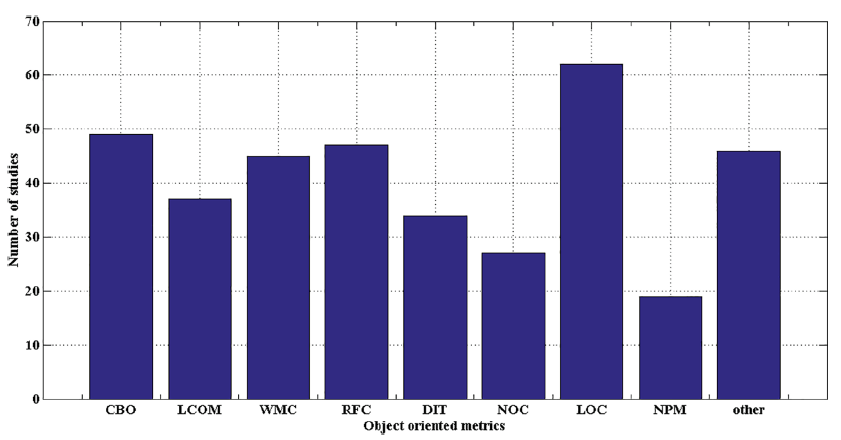
\includegraphics[width=\textwidth]{chapters/ChapterMarcoTeorico/sections/SoftwareMetrics/fig/oometrics.png}
    \setstretch{1} %Interlineado 1
	\captionsetup{labelsep=period, labelfont=bf}
    \caption{Lista de métricas de software orientado a objetos que son útiles para SFP. Tomado desde \cite{PANDEY2021114595}}
    \label{fig:OOmetrics}
\end{figure}
\section{Selección de características}

En \cite{9137899} combinan técnicas simples de eliminación de ruido, distribución desequilibrada de clases y selección de métricas de software para optimizar la predicción de defectos en software. La técnica fue probada en diez conjuntos de datos de predicción de fallos de software. Los resultados experimentales, incluyendo la recall, precisión, medida-F, exactitud y los valores de ROC-AUC, muestran que el método propuesto mejora el rendimiento de la predicción de fallos y los resultados obtenidos son mejores o cercanos a varios modelos comparativos. Se utilizan los conjuntos de datos NASA, Promise, y Github, combinando con los clasificadores: regresión logística, random forest (RF), SVM, naive Bayes.

\begin{figure}[H]
    \centering
    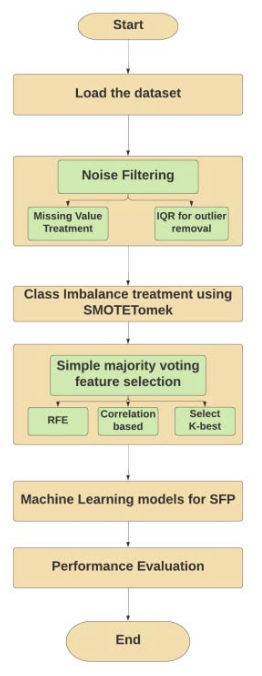
\includegraphics[]{chapters/ChapterMarcoTeorico/sections/FeaturesSelection/fig/Framework defining Methodology adopted for Software Defect.png}
    \setstretch{1} %Interlineado 1
	\captionsetup{labelsep=period, labelfont=bf}
    \caption{Marco que define la metodología adoptada para la predicción de defectos de software. Tomado desde \cite{9137899}}
    \label{fig:Frameworksd}
\end{figure}

En el paso de Selección de Características por Votación Mayoritaria Simple se utiliza un algoritmo de selección de atributos por votación mayoritaria simple para combinar el resultado de tres técnicas de selección de características, es decir, RFECV (eliminación recursiva de características con validación cruzada), selección de características basada en correlación y la técnica de seleccionar las k mejores.

En \cite{kondo2019impact} se utilizan tres Conjuntos de datos (PROMISE,NASA, AEEEM) sumando 26 proyectos en los que varian las metricas y la cantidad de registros.


\section{Datos Desbalanceados}

En la práctica, los modelos de predicción de defectos de software (SDP) a menudo sufren de datos muy desequilibrados, lo que dificulta a los clasificadores identificar instancias defectuosas. Recientemente, se propusieron muchas técnicas para abordar este problema; la técnica de sobremuestreo es uno de los métodos más conocidos para abordar el problema del desequilibrio de clases. Esta técnica equilibra el número de instancias defectuosas y no defectuosas generando nuevas instancias defectuosas.

Motivados por esto en \cite{8861051}, proponemos un enfoque de Sobremuestreo Basado en Clústeres con Filtrado de Ruido (KMFOS) para abordar el problema del desequilibrio de clases en SDP. KMFOS primero divide las instancias defectuosas en $K$ clústeres, y se generan nuevas instancias defectuosas por interpolación entre instancias de cada dos clústeres. Después de esto, estas nuevas instancias defectuosas se dispersarán diversamente en el espacio del conjunto de datos defectuoso. Luego, extendemos este sobremuestreo basado en clústeres mediante la Identificación de Ruido de Lista Cercana (CLNI) para limpiar las instancias de ruido. Realizamos experimentos extensivos en 24 proyectos para comparar KMFOS con algunos enfoques de sobremuestreo como SMOTE, BorderlineSMOTE, ADASYN, sobremuestreo aleatorio (ROS), SMOTE de K-medias, SMOTE + IPF, SMOTE + ENN y SMOTE + Enlaces de Tomek utilizando cinco clasificadores de predicción.
 

\begin{figure}[H]
    \centering
    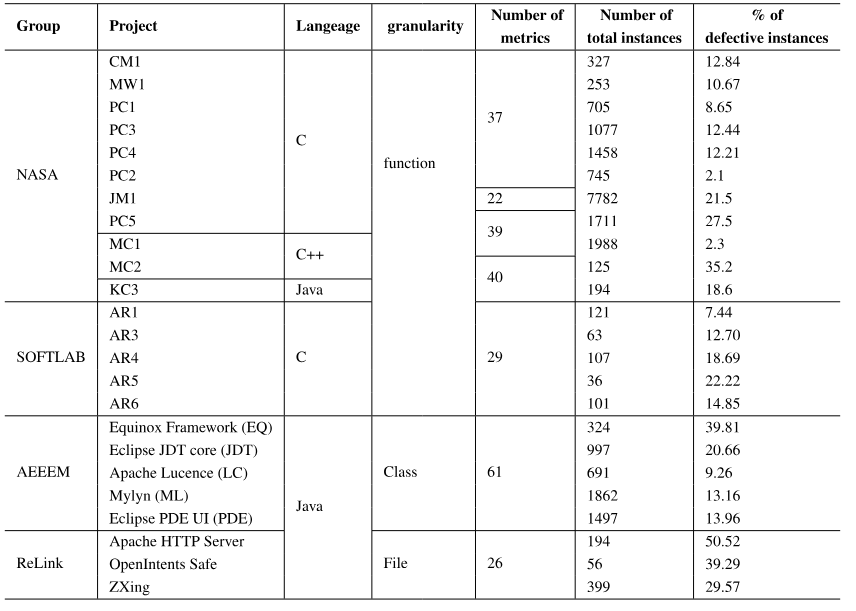
\includegraphics[width=\textwidth]{chapters/ChapterMarcoTeorico/sections/FeaturesSelection/fig/experimental dataset.png}
    \setstretch{1} %Interlineado 1
	\captionsetup{labelsep=period, labelfont=bf}
    \caption{Lista de datasets utilizados. Tomado desde \cite{8861051}}
    \label{fig:desequilibrioDataset}
\end{figure}

De la Figura \ref{fig:desequilibrioDataset}, podemos ver: i) los lenguajes de desarrollo de estos proyectos incluyen Java, C y C++; ii) la granularidad de las métricas cubre función, clase y archivo; iii) el número de instancias varía mucho y la proporción de instancias para la mayoría de los proyectos está muy por debajo del 25\%. Por lo tanto, estos proyectos pueden ser utilizados como objetos experimentales para evaluar estos enfoques con desequilibrio de clases.

En \cite{9044596} se utilizan los proyetos  cm1, kc1, mc2 y pc1 del repositorio PROMISE. Utilizan los clasificadores Logistic regression, NB, Decision tree, MNB y KNN combinados con las tecnicas de remuestreo SMOTE, ROS y RUS.
En la primera fase, aplican las técnicas de remuestreo para todos los clasificadores. En la segunda fase, la combinación de técnica de remuestreo y clasificador que ha tenido mejor desempeño se utiliza en el método de promediación de modelos. Esta combinación sobresaliente se obtiene a partir de las pruebas estadísticas. Su objetivo encontrar el conjunto sobresaliente de clasificador con técnica de remuestreo.




\section{Conjunto de datos}

Según la revisión de Pandey et al. \cite{PANDEY2021114595}, en la investigación sobre SFP se ha utilizado una gran variedad de conjuntos de datos. Su evidencia empírica muestra que el conjunto de datos de la NASA es el más aplicado en la disciplina, seguido de los conjuntos de datos de código abierto y del repositorio PROMISE.


\begin{figure}[H]
    \centering
    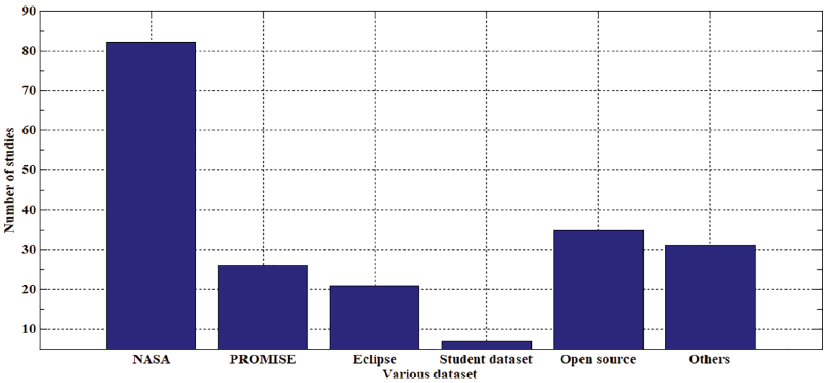
\includegraphics[width=\textwidth]{chapters/ChapterMarcoTeorico/sections/Datasets/fig/SFP dataset.png}
    \setstretch{1} %Interlineado 1
	\captionsetup{labelsep=period, labelfont=bf}
    \caption{Porcentaje de estudios para diferentes conjuntos de datos que se utilizan en SFP. \cite{PANDEY2021114595}}
    \label{fig:SFPDataset}
\end{figure}

Se pueden encontrar algunos patrones en la Figura \ref{fig:datasetdist} en que el conjunto de datos con la distribución de fallos más baja es popularmente utilizado y viceversa. Según el gráfico de barras, los conjuntos de datos de la NASA tienen menos distribución de fallos (CM1, PC1, KC3, MW1, PC4) en comparación con el conjunto de datos del repositorio PROMISE (poi-3.0, lucene-2.4, eclipse-3.0, eclipse-2.1). Una información adicional que informa esta figura es que, en algunos casos, los conjuntos de datos que tienen un gran número de instancias tienen menos distribución de fallos, como JM1. CM1 y JM1 también son conjuntos de datos sustancialmente utilizados que combinan el 57\% de los estudios y contienen el 31\% de los módulos defectuosos.

\begin{figure}[H]
    \centering
    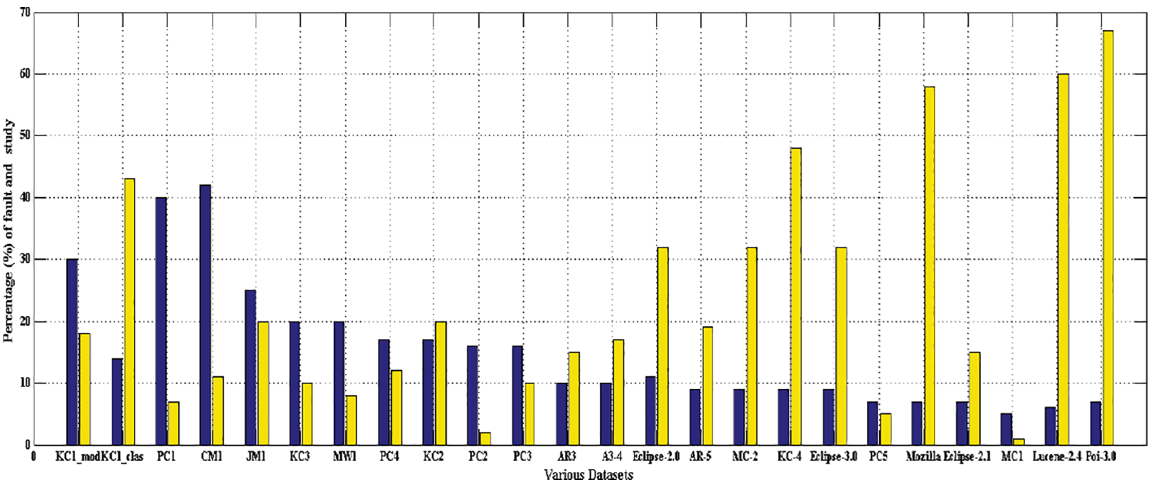
\includegraphics[width=\textwidth]{chapters/ChapterMarcoTeorico/sections/Datasets/fig/datasetdist.png}
    \setstretch{1} %Interlineado 1
	\captionsetup{labelsep=period, labelfont=bf}
    \caption{Distribución de errores de diferentes conjuntos de datos. \cite{PANDEY2021114595}}
    \label{fig:datasetdist}
\end{figure}

\section{Algoritmos utilizados en SFP}
\label{sec:clasificadores_mt}

La predicción de fallas de software (SFP) es una tarea crítica en la ingeniería de software que busca identificar los módulos del software que son propensos a contener defectos. Para realizar esta predicción, se han utilizado varios algoritmos de aprendizaje automático y técnicas estadísticas. A continuación, se describen algunos de los algoritmos más comúnmente utilizados en la literatura para SFP.

\subsubsection{Regresión Logística}
La regresión logística es un método estadístico utilizado para modelar la probabilidad de que una instancia pertenezca a una de dos clases posibles. Este método ha sido ampliamente utilizado en SFP debido a su simplicidad y efectividad para manejar datos binarios. La regresión logística estima la relación entre las variables independientes (métricas del software) y la variable dependiente (presencia o ausencia de defectos) mediante una función logística \cite{kondo2019impact}.

\subsubsection{Máquinas de Vectores de Soporte (SVM)}
Las máquinas de vectores de soporte (SVM) son un conjunto de métodos de aprendizaje supervisado utilizados para clasificación y regresión. Una SVM busca el hiperplano que separa las dos clases con el máximo margen, es decir, con la mayor distancia posible a las instancias más cercanas de cada clase (los vectores de soporte); la formulación de margen suave permite tolerar instancias mal clasificadas mediante un parámetro de penalización \cite{cortes1995}. En su versión lineal, la SVM es rápida de entrenar sobre conjuntos grandes y sensible a la escala de las características, por lo que requiere estandarizarlas previamente. En el contexto de SFP, la SVM ha demostrado ser eficaz para manejar conjuntos de datos de alta dimensionalidad. En esta tesis se utiliza una SVM lineal con estandarización previa como uno de los clasificadores del análisis de sensibilidad.

\subsubsection{Árboles de Decisión}
Los árboles de decisión son modelos de predicción que utilizan un árbol como estructura de decisión y modelan la relación entre las variables de entrada y la variable de salida. Los árboles de decisión, como el algoritmo J48, han sido utilizados en SFP debido a su capacidad para manejar datos categóricos y continuos, y su facilidad de interpretación \cite{RADJENOVIC20131397}.

\subsubsection{Random Forest}
El algoritmo Random Forest \cite{breiman2001} es un conjunto de árboles de decisión, cada uno entrenado sobre una muestra \textit{bootstrap} de las instancias (\textit{bagging}) y considerando en cada división solo un subconjunto aleatorio de las características. La predicción final se obtiene por votación mayoritaria de los árboles. La combinación de ambas fuentes de aleatoriedad reduce la correlación entre árboles y, con ello, la varianza y el riesgo de sobreajuste del modelo \cite{shah_comparative_2020}. Random Forest es uno de los clasificadores más utilizados en SFP y es el clasificador principal de esta tesis, empleado tanto en Weka \cite{weka} como en \textit{scikit-learn}.

\subsubsection{XGBoost}
XGBoost \cite{chen2016} es una implementación escalable del \textit{boosting} de gradiente sobre árboles de decisión. A diferencia de Random Forest, que entrena árboles independientes y promedia sus votos, el \textit{boosting} construye los árboles de forma secuencial: cada nuevo árbol se ajusta para corregir los errores residuales del conjunto acumulado, minimizando una función de pérdida mediante descenso de gradiente con regularización explícita de la complejidad de los árboles. XGBoost representa, por tanto, un paradigma de ensamble distinto al de Random Forest, y se utiliza en el análisis de sensibilidad de esta tesis para verificar que los hallazgos no son específicos de un único clasificador.

\subsubsection{Naive Bayes}
Naive Bayes es un clasificador basado en la teoría de probabilidad bayesiana. Asume la independencia entre las características, lo cual es una simplificación fuerte pero efectiva en muchos casos. En SFP, Naive Bayes ha sido utilizado debido a su simplicidad y eficiencia computacional, especialmente cuando se dispone de grandes conjuntos de datos con múltiples características.

\subsubsection{K-Nearest Neighbors (KNN)}
El algoritmo K-Nearest Neighbors (KNN) es un método de clasificación que asigna una clase a una instancia basándose en las clases de sus k vecinos más cercanos en el espacio de características. KNN ha sido aplicado en SFP debido a su simplicidad y efectividad para capturar relaciones locales en los datos. Sin embargo, puede ser computacionalmente costoso cuando se trabaja con grandes conjuntos de datos.

\subsubsection{Algoritmos de Sobremuestreo y Submuestreo}
Para abordar el problema del desequilibrio de clases en los conjuntos de datos de SFP, se utilizan técnicas de sobremuestreo y submuestreo. Métodos como SMOTE (Synthetic Minority Over-sampling Technique), ROS (Random Over-Sampling), y RUS (Random Under-Sampling) se emplean para equilibrar las clases defectuosas y no defectuosas, con el objetivo de reducir el sesgo del clasificador hacia la clase mayoritaria \cite{9137899,chawla2002}. Su efecto real, sin embargo, depende del contexto experimental y de la métrica de evaluación \cite{8494821}, un aspecto central de esta tesis.

\subsubsection{Modelos de Conjunto}
Los modelos de conjunto, como el Bagging y el Boosting, combinan múltiples clasificadores para mejorar la precisión y la robustez del modelo. Estas técnicas son útiles en SFP para combinar las predicciones de diferentes algoritmos y obtener una mejor estimación de la propensión a fallos de los módulos de software \cite{9044596}.

En resumen, una variedad de algoritmos de aprendizaje automático y técnicas de preprocesamiento se utilizan en la predicción de fallas de software, cada uno con sus propias ventajas y limitaciones. La selección del algoritmo adecuado depende de las características específicas del conjunto de datos y del problema en cuestión.


